%!TEX root = ../document.tex
\chapter{Architecture}\label{ch:architecture}

\begin{quotation}
“Some fantastic quote”
{\small\it --  }
\end{quotation}

This section describes the architecture designed for the browserCloud.js system. browserCloud.js was designed with with the Unix philosophy, that is, subtracting the unnecessary from a subsystem until it is constructed to perform one thing and one thing well, building more cohese abstractions through composition.

browserCloud.js was architectured to meet the following requirements:

\begin{itemize}
    \item \textbf{Membership management} - The system has to enable peers to join and leave a current network of browserCloud.js peers or a subset of it. A peer should only have the knowledge of a small of other peers in the network and be available to rail in any other peer that wants to be part of the P2P network.
    \item \textbf{Message routing} - Peers must have a way to communicate with every other peer in the network without the necessity of contacting a centralized service to do so. Messages should be routed between peers, having each peer knowing a subset of the network, guaranteeing in full coverage in this manner.
    \item \textbf{Job scheduling and results aggregation} - The discovery of computational resources must be performed using a distributed fashing, peers interact between each other to send tasks and retrieve the results for the peer executing the job.
    \item \textbf{Support dynamic runtime} - Provide flexibility for jobs being executed. This is delivered thanks to the dynamic runtime offered by by peers in browserCloud.js due to the fact that they are standard compliant web browsers and Javascript is the language used.
    \item \textbf{Reduced entrance cost to enable greater adoption} - Designed simple APIs, abstracting the complexity in favor of greater extendability.
\end{itemize}

The overview of the network architecture can be seen in Figure~\ref{fig:n-a-o}.

\begin{figure}[h!]
  \centering
  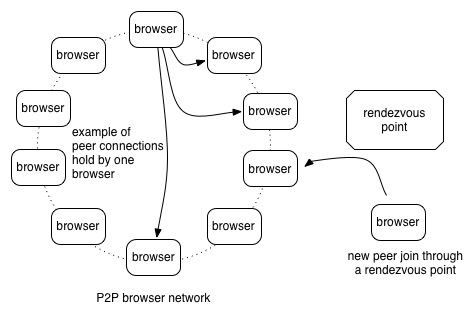
\includegraphics[width=0.7\textwidth]{figs/network-architecture-overview}
  \caption{browserCloud.js Network Architecture Overview}
  \label{fig:n-a-o}
\end{figure}

There are two different kind of actors in the system:

\begin{itemize}
    \item browser - The points on our network that will be able to issue jobs, execute tasks and route messages.
    \item rendezvous point - The only centralized component in this architecture, its purpose is for the clients to have a way to connect to the overlay network. 
\end{itemize}

\section{Interaction design details}

In a browserCloud.js infrastructure, we have three main interaction patterns, the first being when a peer joins or leaves the network, which also we can call membership management, something that in traditionally P2P networks would simply mean an exchange of a pair IP:Port, but in a P2P browser network, a RTCPeerConnection has to be established and kept alive, meaning that an handshaking protocol must be performed. The second pattern is message routing between peers, this has been designed with inspiration on the Chord routing algorithm, studied on the related work. The third interaction demonstrates how to levarage the computer cycles available in the network to process CPU bound jobs.

\subsection{Peer joins and leaves}

A peer join compromisses of the following steps:

\begin{itemize}
    \item \textbf{1 - Registration} - When a peer is ready to join the network, it performs the registration action to the custom browserCloud.js signalling server, the server replies with a confirmation and a unique ID for this peer to occupy in the network. This enables the signalling server, which holds the meta data of the current state in the network, to pick the ID in the ID interval that might be less occupied. We can observe this interaction in Figure~\ref{fig:1-p-r}.
    \item \textbf{2 - New peer available} - As peers join the network, other peers present need to be notified to establish or update their connections to the new best candidates, so that the routing of messages (explained in the next section), remains efficient. For each peer join, a notification of a finger update can be sent to 1 or more peers present, as seen in Figure~\ref{fig:2-p-n}.
    \item \textbf{3 - Connection establishment between two peers} - In order to establish a connection between two peers, once there is an interest for these to connect, for e.g, in the case of a finger update event. There are two substeps, the first being the SDP offer creation through a technique called "hole punching", where a browser uses one of the WebRTC API to traverse through NAT to obtain its public IP, which is crucial information when two browsers need to establish a direction connection, Figure~\ref{fig:3-p-s}. The second step is the exchange of these SDP offers between browsers and that has to be performed by a centralized service, in browserCloud.js we developed a custom signalling server that handles that part, as seen in Figure~\ref{fig:4-p-c}
\end{itemize}

A peer leave is a simplier and organic process, once a peer leaves the network, the RTCPeerConnections objects are destroied, notifying automatically the peers that have to update their finger tables that they should request the signalling server to update the metadata of the state of the network and therefore, issuing new finger-update messages.

The meta state of the network is always hold in memory by the signalling server, there is no need to keep this state persistence because it can be easily reconstructed, in the event of the signalling server failing, a new instance can be spawn and the peers simply have to register again, but this time with their current IDs.

\begin{figure}[h!]
  \centering
  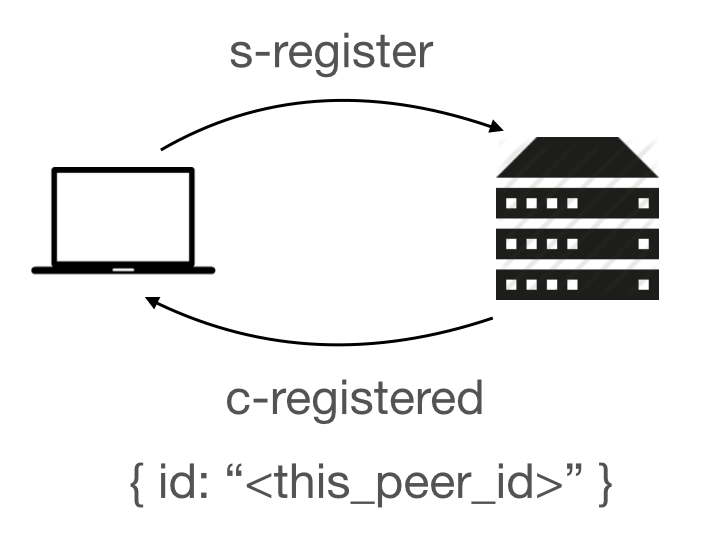
\includegraphics[width=0.4\textwidth]{figs/1-peer-registers}
  \caption{Registration of a peer, signaling itself as available to be part of the P2P network}
  \label{fig:1-p-r}
\end{figure}

\begin{figure}[h!]
  \centering
  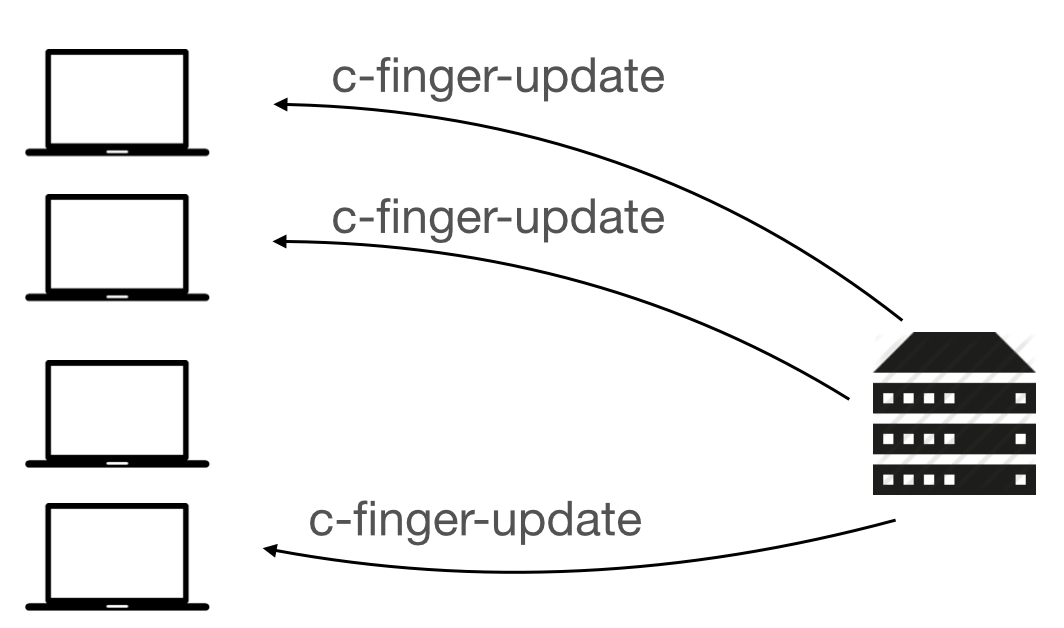
\includegraphics[width=0.4\textwidth]{figs/2-peers-notified}
  \caption{A peer is notified to update his finger table}
  \label{fig:2-p-n}
\end{figure}

\begin{figure}[h!]
  \centering
  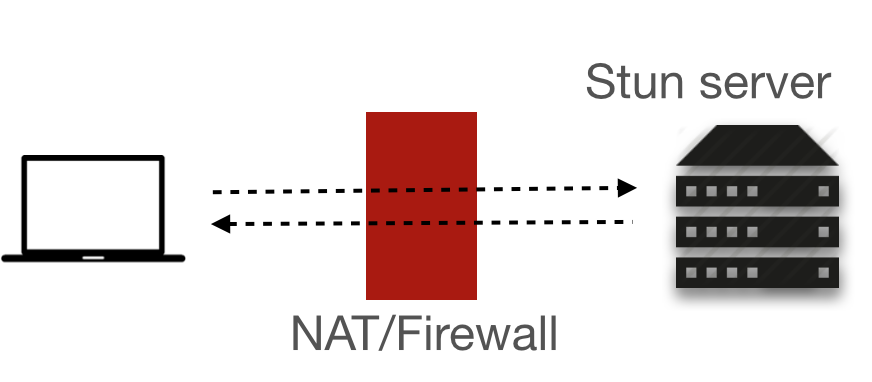
\includegraphics[width=0.4\textwidth]{figs/3-peer-stun}
  \caption{Hole punching through NAT to obtain a public IP and create a SDP offer}
  \label{fig:3-p-s}
\end{figure}

\begin{figure}[h!]
  \centering
  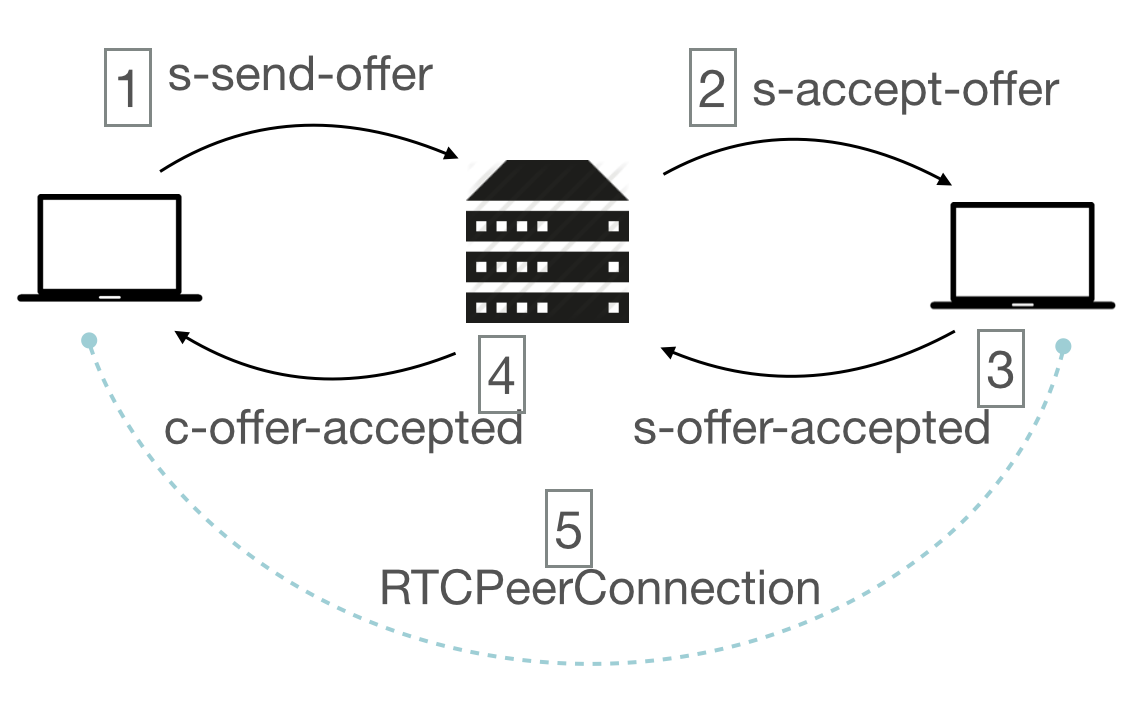
\includegraphics[width=0.4\textwidth]{figs/4-peer-connect}
  \caption{Establishment of a RTCPeerConnection through the custom Signalling Server}
  \label{fig:4-p-c}
\end{figure}


\subsection{Message routing}

"""ON THIS SECTION"""

TODO
Explain CHORD routing
Adaptable finger tables due to expensive Peer Connections

\subsection{Job Scheduling}

Leveraging the browser's dynamic runtime was a feature we pursue from the beginning of the design for browserCloud.js. A job is divided into individual tasks that are a composition of the function to be executed plus the data which should serve as input for that task, creating a transportable gridlet that can be migrated between browsers and executed by its final destination. A job execution is performed as follows:

\begin{itemize}
    \item 1 - Select in how many units we want to divide a job.
    \item 2 - Select how many browsers we want to distribute the job to.
    \item 3 - Query the network for browser available (e.g. that are not performing other jobs at the moment).
    \item 4 - Compose the several units (gridlets) with with task plus data partition.
    \item 5 - Send this gridlets to the network to be routed to the browser that is going to execute them.
    \item 6 - browser compute the results and send them back to the job issuer.
    \item 7 - the browser that submited the job gathers all the tasks results and constructs the job result.
\end{itemize}

\section{Architecture of the Software stack}

When it comes to software, we divided our browser application appliance into three separate and fundamental components, namely: Communication layer, Service router and Job scheduler, leaving also the opportunity for these to be extended. We can observe a overview of this architecture in Figure~\ref{fig:s-a-n-l}.

\begin{figure}[h!]
  \centering
  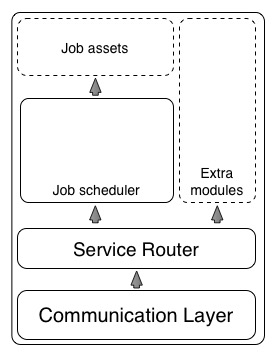
\includegraphics[width=0.4\textwidth]{figs/software-architecture-node-level}
  \caption{Software layers at the peer level}
  \label{fig:s-a-n-l}
\end{figure}


\subsection{Communication layer}

The communication layer is responsible for routing messages between peers and establish a connection with the rendezvous point to perform a peer join/leave. This means that the communication layer:

\begin{itemize}
    \item Holds the connections with other peers.
    \item Performs the necessarity logic for efficient routing.
    \item Keeps the peer connected to the network by updating its routing table as necessary
\end{itemize}

\subsection{Service router}

The Service router establishes a protocol for modules like the job scheduler to interact with the network of peers, it uses an event driven model, where modules can register listeners to events that happen on the network (such as a specific reception of a message) and react to it. It also offers the necessary API calls for the modules to send messages to the network.

Service router offers extensibility to browserCloud.js, similar to Job scheduler, other modules can be implemented to interact with the already established P2P network.

\subsection{Job scheduler}

The Job scheduler benefits the API of the Service router to implement its logic, this means that although a job scheduler was implemented to fit our design purposes, it could easily be replaced by another job scheduler with different offers and guarantees.

A job consists in the partition of tasks which are enriched with data and sent to other peers to be executed, this tasks, which can be represented as functions (job assets), can be defined in runtime, therefore giving a greater flexibility to the developer that is using this system to run the distributed job they want.

\section{API design details}

For the user of browserCloud.js, a simple API was created to perform: peer join, message listening and job scheduling as demonstrated by the following code (which should be interpreted as pseudo-code since the API might change with the release of new versions):

\textit{Peer join}
\begingroup
\scriptsize
\begin{verbatim}
    // browserCloud.js browser module name is called webrtc-explorer.

    var Explorer = require('webrtc-explorer'); 
    
    var config = {
        signalingURL: '<signalling server URL>'
    };

    var peer = new Explorer(config);

    peer.events.on('registered', function(data) {
        console.log('registered with Id:', data.peerId);
    });

    peer.events.on('ready', function() {
        console.log('ready to send messages');
    });

    peer.register();
\end{verbatim}
\endgroup


\textit{Listen for messages}
\begingroup
\scriptsize
\begin{verbatim}
    // The only action that has to be performed is listen for the message event 
    peer.events.on('message', function(envelope) {
        console.log(envelope);
    });
\end{verbatim}
\endgroup


\textit{Execute a job}
\begingroup
\scriptsize
\begin{verbatim}
    var browserProcess = require('webrtc-explorer-browser-process');

    var config = {
        signalingURL: 'http://localhost:9000'
    };
    
    // Make this browser available to execute tasks and also prepared to issue jobs to the network
    browserProcess.participate(config);

    var start = function() {
        var data = [0,1,2,3,4,5,6,7,8,9,10];  // simple data input
        var task = function(a) {return a+1;}; // e.g of a task (
        var nPeers = 2; // number of peers we are requesting from the network to execute our job
        
        browserProcess.execute(data, task, nPeers, function done(result){
            console.log('Received the final result: ', result); 
        });
    };
\end{verbatim}
\endgroup

\section{Summary}

In this section, we covered the network topology of browserCloud.js, which and how interactions are performed and how a developer can use this system.
